\documentclass[tikz,border=5pt]{standalone}
\usepackage{amssymb,amsmath}
\usepackage{tikz}
\usepackage{lmodern}
\usetikzlibrary{calc}

\begin{document}
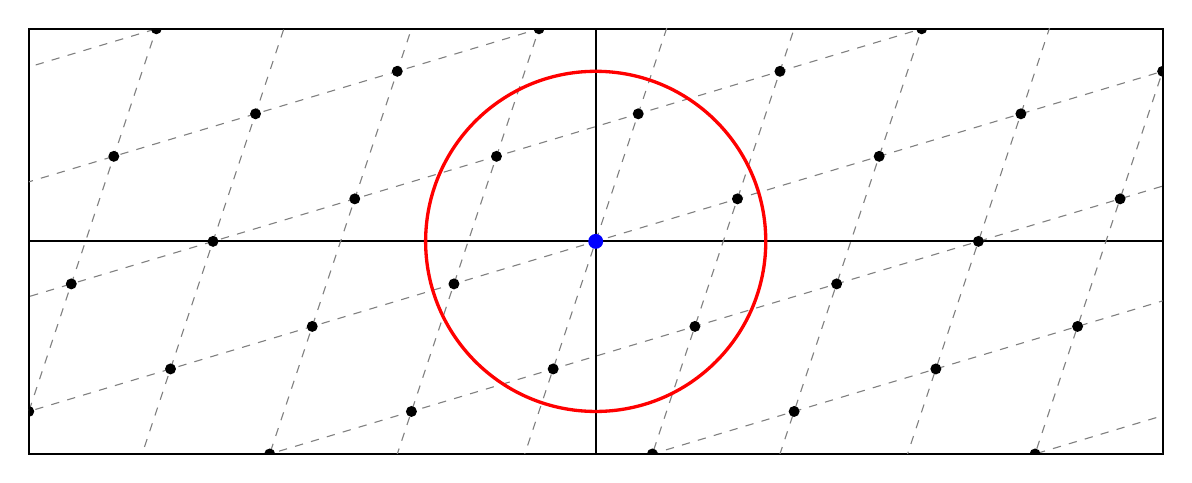
\begin{tikzpicture}[scale=0.9]
	
	% ---- (A) parameters you can easily change ----
	\def\xmin{-8}
	\def\xmax{ 8}
	\def\ymin{-3}
	\def\ymax{ 3}
	
	% basis vectors (change these to change the slant)
	\def\bax{2.0}   % b1 = (bax, bay)
	\def\bay{0.6}
	\def\bbx{0.6}   % b2 = (bbx, bby)
	\def\bby{1.8}
	
	% circle radius
	\def\R{2.4}
	
	% ---- (B) border (optional) ----
	\draw[thick] (\xmin,\ymin) rectangle (\xmax,\ymax);
	
	% clip everything to the box
	\begin{scope}
		\clip (\xmin,\ymin) rectangle (\xmax,\ymax);
		
		% ---- (C) axes ----
		\draw[thick] (\xmin,0) -- (\xmax,0);
		\draw[thick] (0,\ymin) -- (0,\ymax);
		
		% ---- (D) dashed parallel lines (two directions) ----
		% Lines parallel to b1, shifted by multiples of b2
		\foreach \k in {-6,-5,...,6}{
			% a point on the line: k*b2
			\pgfmathsetmacro{\px}{\k*\bbx}
			\pgfmathsetmacro{\py}{\k*\bby}
			% draw long segment in direction b1 through that point
			\draw[gray, dashed]
			({\px-20*\bax},{\py-20*\bay}) -- ({\px+20*\bax},{\py+20*\bay});
		}
		
		% Lines parallel to b2, shifted by multiples of b1
		\foreach \k in {-6,-5,...,6}{
			% a point on the line: k*b1
			\pgfmathsetmacro{\qx}{\k*\bax}
			\pgfmathsetmacro{\qy}{\k*\bay}
			% draw long segment in direction b2 through that point
			\draw[gray, dashed]
			({\qx-20*\bbx},{\qy-20*\bby}) -- ({\qx+20*\bbx},{\qy+20*\bby});
		}
		
		% ---- (E) lattice points: i*b1 + j*b2 ----
		\foreach \i in {-6,-5,...,6}{
			\foreach \j in {-6,-5,...,6}{
				\pgfmathsetmacro{\x}{\i*\bax+\j*\bbx}
				\pgfmathsetmacro{\y}{\i*\bay+\j*\bby}
				\fill (\x,\y) circle (2.2pt);
			}
		}
		
		% ---- (F) red circle and blue center point ----
		\draw[red, very thick] (0,0) circle (\R);
		\fill[blue] (0,0) circle (3pt);
		
	\end{scope}
\end{tikzpicture}
\end{document}